\documentclass[a4paper, 12pt]{article}

\usepackage[T1]{fontenc}

\usepackage{lipsum}
\usepackage{pifont}
\usepackage{amssymb}

\usepackage[utf8]{inputenc}
\usepackage[italian]{babel}
\usepackage{graphicx}
\graphicspath{ {./images/} }
\usepackage{spverbatim}
\usepackage{float}
\usepackage{url}
\usepackage{hyperref}

\usepackage{xcolor}
\definecolor{linkcolor}{RGB}{1,1,87}
\hypersetup{
    colorlinks,
    citecolor=black,
    filecolor=black,
    linkcolor=linkcolor,
    urlcolor=black
}

\usepackage{xstring}



\newcommand{\e}[1]{\texttt{\StrSubstitute{#1}{_}{\_}}}
\newcommand{\Null}[0]{\e{NULL}}
\newcommand{\nota}[1]{\textbf{Nota}: #1}
\newcommand{\tbs}[0]{\textbackslash}




\newcommand{\makesub}[1]{%
  \saveexpandmode\noexpandarg
  \StrSubstitute{#1}{\_}{_}[\temp]%
  \restoreexpandmode
}
\newcommand{\target}[1]{%
  \makesub{#1}%
  \hypertarget{\temp}{}%
}
\newcommand{\attach}[1]{%
  \makesub{#1}%
  \hyperlink{\temp}{\e{#1}}%
}


\newcommand{\func}[1]{%
	\attach{#1}%
}




\begin{document}\sloppy
  
\title{
  \textbf{
    \emph{Relazione homework 1}
  }
}  
\author{Luca Mastrobattista}
\date{}
\maketitle

\tableofcontents

\newpage
\section{Traccia dell'homework}
\subsection{Testo}
Analizzare con Ghidra, utilizzando lo strumento 
disassemblatore / decompilatore, il programma eseguibile
hw1.exe contenuto nell'archivio hw1.zip (password: "AMW21").
Riassumere in un documento tutte le informazioni acquisite
sul programma, con particolare riguardo alle strutture di
dati fondamentali utilizzate.
Descrivere anche la metodologia ed i passi logici deduttivi
utilizzati nel lavoro di analisi.
\subsection{Scadenza}
Due settimane dalla data di assegnazione del lavoro: 28/10/2021
\subsection{Consegna}
Documento in formato PDF inviato come allegato ad
un messaggio di posta elettronica all'indirizzo del docente
("$<$cognome$>$@uniroma2.it"), con subject:
"[AMW21] HW1: $<$matricola studente$>$"

\newpage
\section{Ambiente di lavoro}
Il file eseguibile è stato caricato su Ghidra istallato su un sistema operativo Linux. 

\newpage
\section{Metodologia}

\subsection{Informazioni note a priori}
Eseguibile ottenuto per l'esecuzione dell'homework e, quindi, non sono note informazioni preliminari.

\subsection{Finalizzazione dell'obiettivo}
Il reversing dell'applicazione ha come obiettivo quello di comprendere il funzionamento dell'eseguibile e di completare l'attività di e{reverse code engineering}, quindi l'obiettivo dello studio è la ricostruzione dell'intero programma.

\subsection{Ottenimento del codice macchina}
Codice macchina fornito dal professore.


\subsection{Osservazione del funzionamento}
Provando ad eseguire l'eseguibile su una macchina virtuale del sistema operativo Windows 10 non è stato ottenuto alcun output. Neanche nel gestore attività viene riportata alcuna informazione. L'applicazione sembra avviarsi e terminare in poco tempo.\newline

\begin{figure}[H]
\centering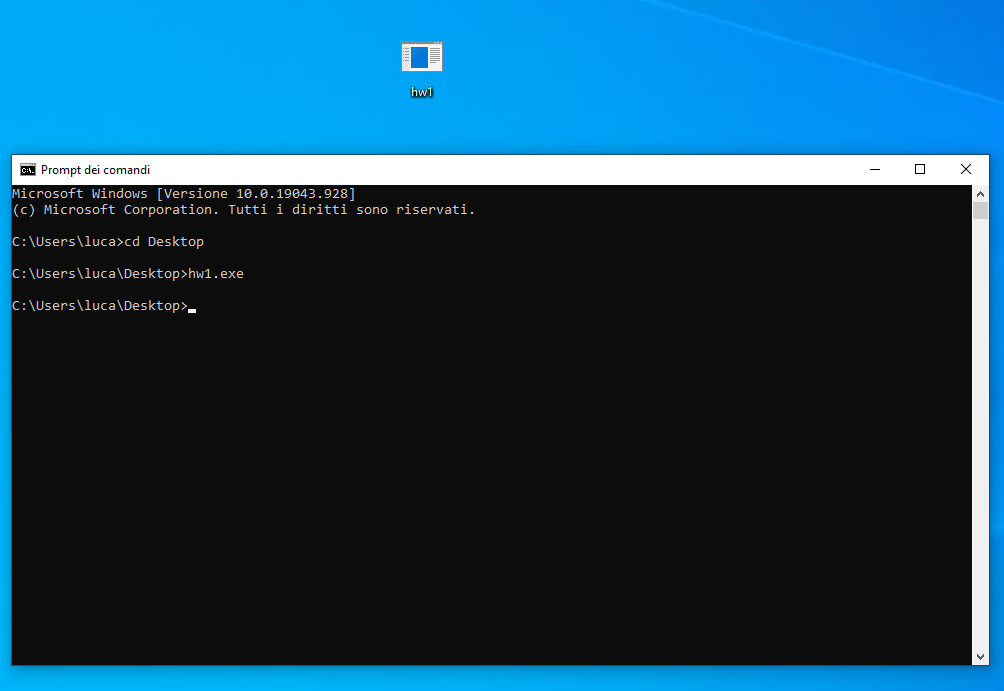
\includegraphics[width=\textwidth]{esecution}
\end{figure}

\subsection{Disassemblaggio del codice macchina}
Lo strumento che si è utilizzato è il software \emph{Ghidra}.

\subsubsection{Riepilogo risultati dell'import}
\begin{figure}[H]
\centering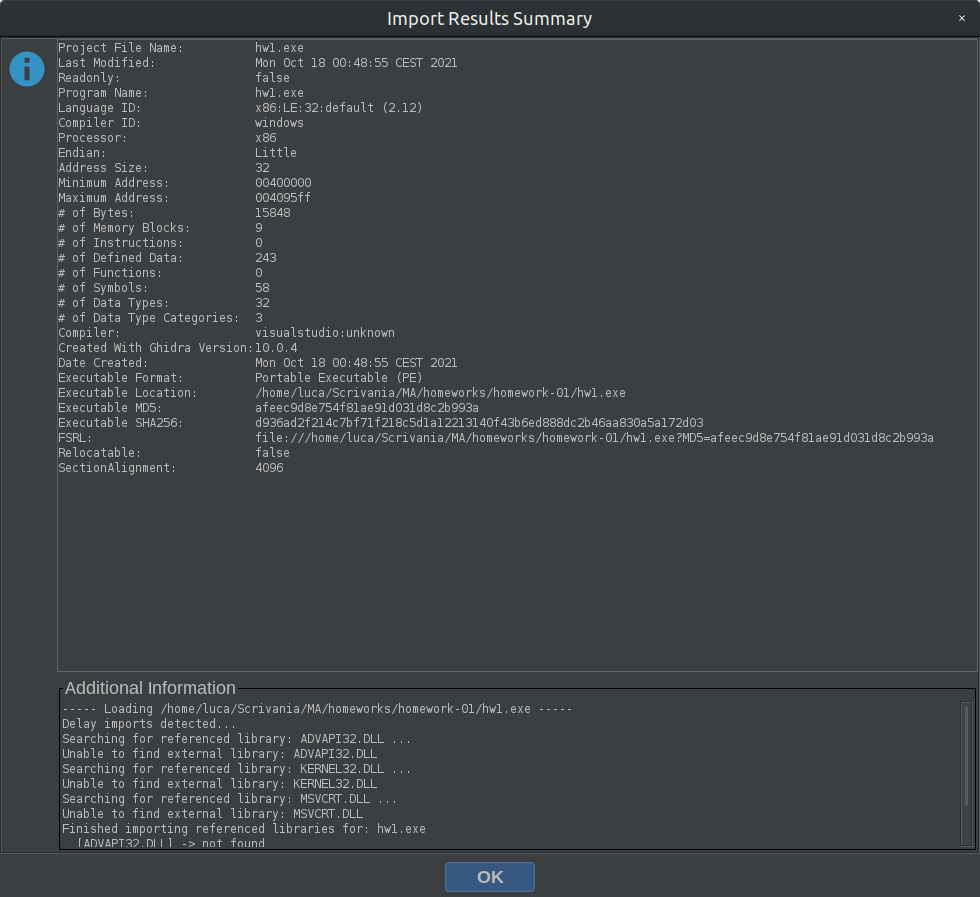
\includegraphics[width=\textwidth]{Import_Results_Summary}
\end{figure}

\subsubsection{Informazioni aggiuntive}
\begin{spverbatim}

----- Loading /home/luca/Scrivania/MA/homeworks/homework-01/hw1.exe ----- 
Delay imports detected... 
Searching for referenced library: ADVAPI32.DLL ... 
Unable to find external library: ADVAPI32.DLL 
Searching for referenced library: KERNEL32.DLL ... 
Unable to find external library: KERNEL32.DLL 
Searching for referenced library: MSVCRT.DLL ... 
Unable to find external library: MSVCRT.DLL 
Finished importing referenced libraries for: hw1.exe 
  [ADVAPI32.DLL] -> not found 
  [KERNEL32.DLL] -> not found 
  [MSVCRT.DLL] -> not found 
\end{spverbatim}

\newpage
\subsection{Ricerca del main}
\subsubsection{Ricerca tramite invocazioni di funzioni user}
Tentativo di ricerca del \e{main} sfruttando le invocazioni a funzioni di libreria. Nella libreria \e{MSVCRT.DLL} viene invocata la funzione \e{printf}. Cercando le referenze a quest'ultima, ne sono state trovate 7. Queste invocazioni sono tutte all'interno della stessa funzione: \func{FUN_00401790}. Questa funzione, però, non può essere il nostro \e{main}, perché prende in input un parametro che viene usato per indicizzare elementi da passare alle varie \e{printf}. Tra i vari elementi indicizzati, cerca di prendere anche \e{param_1[0xc]}; questa istruzione viene eseguita sempre, e perciò avrebbe dovuto sollevare un errore in caso di avvio dell'applicazione senza parametri. Inoltre, proprio questo valore \e{param_1[0xc]} è usato per indicizzare a sua volta un indirizzo con un offset di \e{0x400c}, corrispondente  a \e{16396}. Infine, questa funzione non viene invocata da \e{entry}, ma da un'altra funzione definita dal programmatore. È quindi difficile credere che \e{param_1} sia un vettore di stringhe, ma è più probabile che sia una struttura dati più complessa.\\
In ogni caso, si può essere sicuri che questa funzione sia stata definita dal programmatore, e in questo modo è possibile sfruttare il grafo delle invocazioni delle funzioni per risalire al \e{main}.
\begin{figure}[H]
	\centering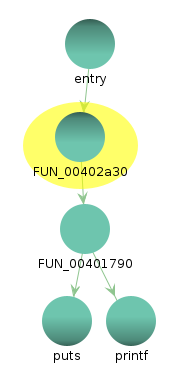
\includegraphics[scale=0.6]{main_ipotetic_tree}\newline
	 La funzione \func{FUN_00402a30} è un buon canditato ad essere il main.
\end{figure}
Una conferma che quella funzione sia effettivamente il \e{main} arriva dalla seguente osservazione. Nella funzione \e{entry}, viene invocata due volte la funzione \e{MSVCRT.DLL::_initterm}, che prende in input due puntatori. Questi puntatori identificano l'inizio e la fine di una tabella di puntatori a funzioni e vengono inizializzati. Delle due invocazioni, è interessante la seconda: gli indirizzi dati in input identificano una tabella di un solo puntatore a funzione che, una volta definito tale, punta alla \emph{LAB\_00401120} che va quindi definita come funzione. Al suo interno viene invocata la funzione \e{MSVCRT.DLL::__getmainargs}. Questa funzione richiama l'analisi della riga di comando e copia gli argomenti del \e{main}. Riceve in input 5 paremetri che sono tutti variabili globali e rappresentano, in ordine:
\begin{itemize}
\item L'intero \e{argc}
\item La amtrice di stringe \e{argv}
\item Una matrice di stringe \e{_env} che rappresenta le variabili impostate nell'ambiente dell'utente.
\item Un intero che, e impostato su 1, espande i caratteri jolly negli argomenti della riga di comando o, se impostato su 0, non esegue alcuna operazione.
\item Un puntatore a \e{_startupinfo}, che contiene altre informazioni da passare alla DLL CRT.
\end{itemize}
La cosa interessante è che i primi due parametri sono passati in input anche alla funzione \func{FUN_00402a30}, proprio in quell'ordine: quella funzione prende in input \e{argc} e \e{argv}, e non può che essere il \e{main}. 



\begin{figure}[H]
\emph{Function call graph del main prima dell'analisi}
\centering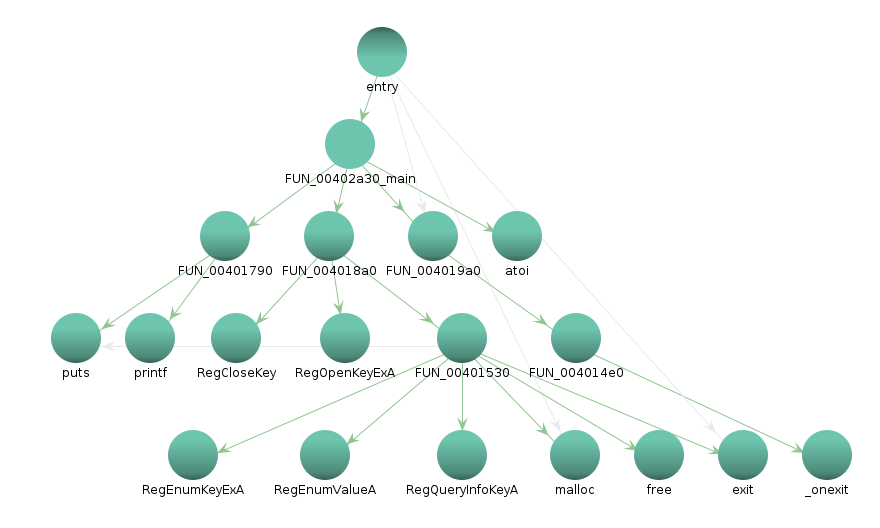
\includegraphics[width=\textwidth]{main_call_graph_pre_analisi}\\
\end{figure}

\begin{figure}[H]
\emph{Function call graph del main dopo l'analisi}
\centering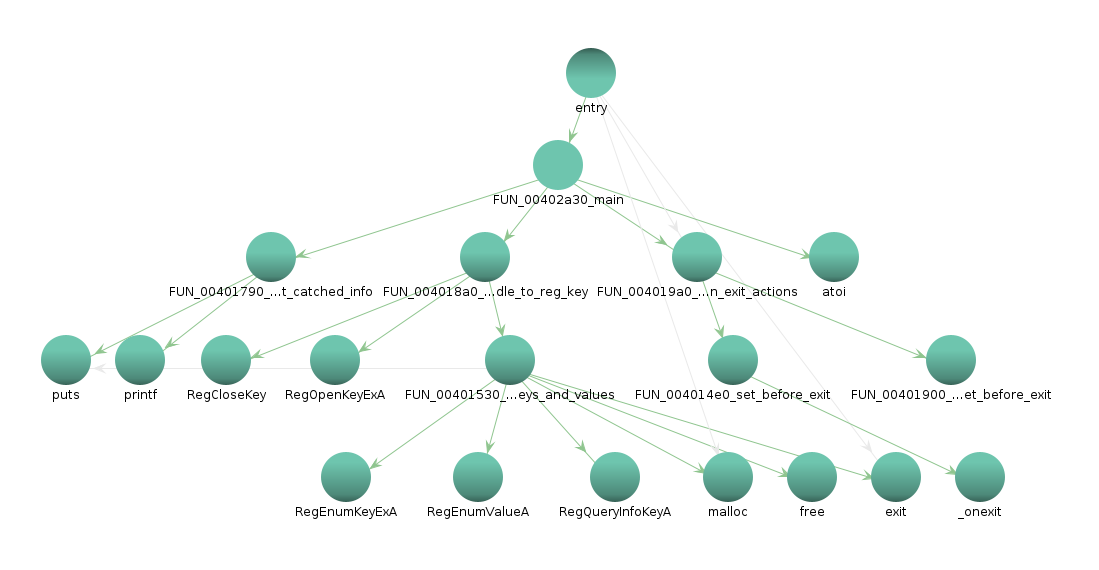
\includegraphics[width=\textwidth]{main_call_graph}\\
\end{figure}


\newpage
\section{Analisi con Ghidra}

\target{FUN\_00402a30\_main}
\target{FUN\_00402a30}
\subsection{FUN\_00402a30\_main}

Questa funzione, dopo aver fatto allineamento a 16 bytes, ne invoca subito un'altra: \func{FUN_004019a0_set_on_exit_actions}, analizzata in seguito.\\
Poi continua con dei controlli sulla riga comando: effettua \e{argv[argc]} e il risultato viene utilizzato per fare dei controlli. In particolare, se il valore così indicizzato è \Null{}, la funzione ritorna 0, altrimenti verifica il numero dei parametri passati: se è minore di 3, incluso il nome del programma, si imposta a \Null{} il valore di \e{argv[1]} e di \e{argv[2]}. Poi prepara l'invocazione di \e{MSVCRT.DLL::atoi}, che prende in input una stringa e ne restituisci il valore decimale rappresentato. La stringa data in input è il primo parametro a riga comando. Se il valore di ritorno è 0, si memorizza il valore della macro \e{HKEY_LOCAL_MACHINE} in \e{EAX}. Si continua controllando il secondo parametro a riga comando: se è \Null{} si salva in \e{EDX} il valore della stringa \e{"SYSTEM\string\\ControlSet001\string\\Control"}. Questi due registri conterranno i parametri da passare all'invocazione di \func{FUN_004018a0_open_handle_to_reg_key}. Dopo l'invocazione, si controlla il valore ritornato dalla funzione: se è 0, termina, altrimenti salva questo valore nello stack e invoca la funzione \func{FUN_004018a0_open_handle_to_reg_key}. Quando quest'ultima termina, viene ritornato il valore 0.\\

\nota{il primo controllo che viene fatto è:}
\begin{verbatim}
if (argv[argc] == (char *) 0)
    uvar4 = 0;
else{
	...
}
return uvar4	
\end{verbatim}
Ma la condizione dell'\texttt{if} è sempre vera: infatti, se al programma sono dati $argc$ parametri, l' $argc-esimo$ sarà sempre \Null{}.



\target{FUN\_004019a0\_set\_on\_exit\_actions}
\subsection{FUN\_004019a0\_set\_on\_exit\_actions}

La funzione prende il valore della variabile globale \e{DWORD_00405020_one_time_control_label} e controlla se è 0: se non lo è, termina, altrimenti continua impostandolo a 1. Sembra quindi essere una variabile di controllo per evitare che questo codice venga eseguito più di una volta: infatti gli unici riferimenti a questa variabile sono all'interno di questa funzione. Ha senso perché questa funzione è invocata anche dentro \e{entry}. Dopodiché, controlla il valore di un'altra variabile, \e{DAT_00402ac0_my_struct}. In particolare, viene controllato se il suo valore è uguale a -1. Se non lo è, azzera il registro \e{EAX} con un'istruzione di \e{XOR}, e inizia un ciclo. Ad ogni iterazione, il valore di \e{EAX} viene prima salvato in \e{EBX}, poi incrementato di 1, poi moltiplicato per 4 e infine viene usato come offset dal punto base fissato all'indirizzo di \e{DAT_00402ac0_my_struct}. Questo fatto lascia pensare che, in quell'indirizzo, sia memorizzata una struttura dati con componenti tutti della stessa taglia; potrebbe, a questo punto, essere anche un array di interi: sappiamo infatti che il primo elemento è stato confrontato col valore -1. \\
Il ciclo termina quando viene trovato un offset, multiplo di 4 byte, che indicizza \e{NULL} a partire da \e{DAT_00402ac0_my_struct}. Alla fine di questo ciclo, in \e{EBX} è memorizzato il numero di indirizzi diversi da \e{NULL} successivi a \e{DAT_00402ac0_my_struct}. Se questo valore è diverso da 0, cioè si è trovato almeno un indirizzo valido, parte un altro ciclo in cui vengono effettuate delle \e{CALL}. Le funzioni invocate sono tutte quelle memorizzate negli indirizzi che sono diversi da \e{NULL} trovati precedentemente. \\
A questo punto, la nostra \e{my\_struct} è definita così:
\begin{figure}[H]
\centering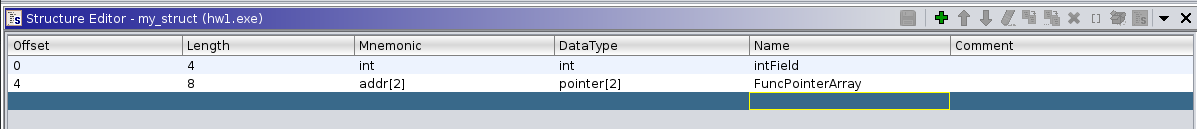
\includegraphics[width=\textwidth]{my_struct}\\
\end{figure}
Il vettore di puntatori a funzioni è definito di dimensione 2 perché è il minimo valore che permette di avere una funzione da invocare e il \Null{} per indicarne la fine. A questo punto dell'analisi non è nota la sua dimensione reale. Inoltre, la struttura dati all'indirizzo \e{DAT_00402ac0_my_struct}, contiene un intero al primo campo, l'indirizzo della funzione \func{FUN_00401500_in_my_struct}, e poi un \Null{}: effettivamente l'array ha solo 2 elementi. \\

Quando queste invocazioni terminano e il ciclo finisce, la funzione inserisce l'indirizzo di una funzione nello stack (\func{FUN_00401900_given_to_set_before_exit}), alla posizione \e{-0x1c} e invocherà poi \func{FUN_004014e0_set_before_exit} prima di terminare.\\

\nota{lo stack pointer viene cambiato come prima istruzione di \func{FUN_004014e0_set_before_exit}, che alloca proprio \e{0x1c} bytes; quindi il primo parametro di quella funzione corrisponderà al valore inserito in questo offset.}


\target{FUN\_00401500\_in\_my\_struct}
\subsection{FUN\_00401500\_in\_my\_struct}
Questa funzione era marcata come \e{UndefinedFunction} dal decompilatore perché non viene trovata una \e{CALL} che invoca direttamente questa funzione ed è l'unica presente nell'array di vettori nell'istanza di \e{my_struct} all'indirizzo \e{DAT_00402ac0_my_struct}. L'unica cosa che fa è invocare \func{FUN_004014e0_set_before_exit}, a cui viene passato in input il valore di \e{DAT_00401520}. Poiché, come vedremo, \func{FUN_004014e0_set_before_exit} prende in input un puntatore a funzione, possiamo dedurre che il valore della variabile \e{DAT_00401520} è un puntatore a funzione.\\

\textbf{Problema}: convertendo la variabile \e{DAT_00401520} in tipo di dato \emph{pointer}, viene indicizzato un indirizzo che non è presente nell'address space. Tuttavia questo valore è passato a \e{_onexit}, che prende in input un puntatore a funzione e non può quindi essere di un altro tipo.

\target{FUN\_00401900\_given\_to\_set\_before\_exit}
\subsection{FUN\_00401900\_given\_to\_set\_before\_exit}

Questa funzione, per prima cosa, carica un indirizzo dentro il registro \e{EAX}. Questo indirizzo, chiamato \e{PTR_PTR_00403004}, è un puntatore doppio. Infatti, subito dopo, viene preso l'indirizzo puntato e si controlla se questo sia \Null{}. Se lo è, termina, altrimenti inizia un ciclo che, come prima istruzione, prevede una \e{CALL} proprio a quell'indirizzo. Di conseguenza, il valore puntato da \e{PTR_DAT_00403004} è un puntatore a funzione. \\
Nelle iterazioni si sposta di 4 bytes in avanti rispetto all' ultimo indirizzo usato nella \e{CALL} e, se non è \Null{}, procede con la sua invocazione. Si sta praticamente scorrendo un ipotetico array di puntatori a funzioni. Il ciclo termina quando viene trovato un puntatore a \Null{}; quando ciò accade la funzione ritorna.\\

\target{Nota}
\nota{il primo controllo che viene fatto è che l'indirizzo base puntato da \e{PTR_PTR_00403004} non sia \Null{}, ma nel codice questo puntatore punta proprio a \Null{}. La funzione dovrebbe quindi terminare semplicemente, senza fare altro.}

\target{FUN\_004014e0\_set\_before\_exit}
\subsection{FUN\_004014e0\_set\_before\_exit}
Questa funzione invoca al suo interno la funzione di libreria \e{MSVCRT.DLL::_onexit}. Questa funzione prende in input un puntatore alla funzione che deve essere invocata prima che il programma termini, una sorta di \e{wrapper} per l'evento di uscita. In caso di più invocazioni di questa funzione, l'ordine di esecuzione delle varie funzioni è quello \emph{LIFO}: infatti la documentazione riporta il seguente esempio:
\begin{verbatim}

#include <stdlib.h>
#include <stdio.h>

/* Prototypes */
int fn1(void), fn2(void), fn3(void), fn4 (void);

int main( void )
{
   _onexit( fn1 );
   _onexit( fn2 );
   printf( "This is executed first.\n" );
}

int fn1()
{
   printf( "executed next.\n" );
   return 0;
}

int fn2()
{
   printf( "This is " );
   return 0;
}

\end{verbatim}
L'output è: 
\begin{verbatim}
This is executed first.
This is executed next.
\end{verbatim} \bigskip 

È utile quindi ricercare tutti i punti in cui questa funzione viene invocata. Ci sono solo 2 riferimenti, entrambi nella funzione \func{FUN_004019a0_set_on_exit_actions}: uno è diretto, l'altro invece è nascosto: si invoca tramite la struttura dati \e{my_struct}
\begin{figure}[H]
\centering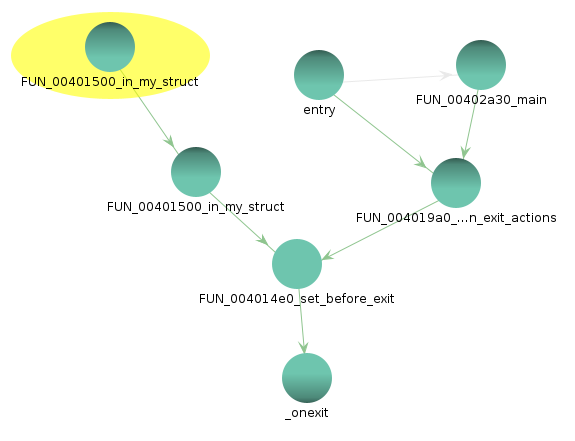
\includegraphics[scale=0.4]{set_before_exit} \\
\nota{la funzione \func{FUN_00401500_in_my_struct} compare 2 volte perchè la prima, quella evidenziata nell'immagine, è una \emph{Thunk}.}
\end{figure} \bigskip

Prima di terminare l'applicazione, quindi, le funzioni verrano eseguite nel seguente ordine:
\begin{enumerate}
\item \func{FUN_00401900_given_to_set_before_exit}, che però, come detto, nella \func{Nota}, dovrebbe terminare subito.
\item \func{FUN_00401500_in_my_struct}, che però utiliza un indirizzo non presente nell'address space: \e{PTR_DAT_00401520} ha come valore \e{DAT_909090c3}, segnato in rosso da Ghidra.
\end{enumerate}
Nessuna funzione viene impostata come \emph{wrapper} per l'evento di \emph{exit}.


\target{FUN\_004018a0\_open\_handle\_to\_reg\_key}
\subsection{FUN\_004018a0\_open\_handle\_to\_reg\_key}
Questa è un'altra funzione invocata da \e{main} che, per prima cosa, azzera il registro \e{EBX}, poi prepara l'invocazione di \e{ADVAPI32.DLL::RegOpenKeyExA}. Questa funzione prende in input i seguenti parametri:
\begin{enumerate}
\item un \e{HKEY}, passato in input alla funzione;
\item un \e{LPCSTR}, anche questo dato in input alla funzione
\item un \e{DWORD}, che in questo caso è 0;
\item un \e{REGSAM}, una maschera di bit che rappresenta i diritti di accesso, e in questo caso è impostato a \e{0xf003f} che corrisponde a \e{KEY_ALL_ACCESS};
\item un \e{PHKEY}, un puntatore che riceve l'handle verso la key aperta.
\end{enumerate} 
Quando la funzione ritorna, si controlla il suo valore di ritorno: infatti, se tutto è andato bene, ritorna il valore 0, corrispondente a \e{ERROR_SUCCESS}. Se in \e{EAX} c'è effettivamente il valore 0, si mette sullo stack l'handle verso la key aperta e si invoca \func{FUN_00401530_retrieve_subkeys_and_values}. Il valore di ritorno di questa funzione si memorizza in \e{EBX}. Poi si invoca \e{ADVAPI32.DLL::RegCloseKey}, passandogli come parametro l'handle verso la key ottenuto precedentemente, in modo da chiuderlo. Infine, la funzione termina restituendo il valore contenuto in \e{EBX}, che sarà \Null{} se c'è stato un errore oppure il risultato di \func{FUN_00401530_retrieve_subkeys_and_values}. \bigskip

\emph{Riassumendo}: si apre il \emph{registry key path} dato da riga comando ottenendo un \emph{handle} verso il registro tramite l'invocazione di \e{ADVAPI32.DLL::RegOpenKeyExA}; se non viene passato nulla, il default è impostato a: \e{HKEY_LOCAL_MACHINE\tbs{}SYSTEM\tbs{}ControlSet001\tbs{}Control} . Si invoca poi  \func{FUN_00401530_retrieve_subkeys_and_values} passandogli l'handle ottenuto, il cui valore di ritorno viene passato al \e{main} dopo aver chiuso l'\emph{handle} con \e{ADVAPI32.DLL::RegCloseKey}.

\target{FUN\_00401530\_retrieve\_subkeys\_and\_values}
\subsection{FUN\_00401530\_retrieve\_subkeys\_and\_values}
La prima cosa che fa questa funzione è allocare 52 bytes con un'invocazione di \e{MSVCRT.DLL::malloc}. Quindi viene controllato il valore di ritorno di questa invocazione e, se è \Null{}, viene invocata una \e{MSVCRT.DLL::puts} per stampare la stringa \e{"Memory allocation error"} prima di terminare con una chiamata a \e{MSVCRT.DLL::exit}, con \emph{exit code} pari a 1.\\
Se le cose vanno bene, invece, si salva il valore ritornato dentro il registro \e{EBX}. Si invoca poi una nuova \e{malloc} per allocare 260 bytes. Anche qui, si controlla il valore di ritorno e si eseguono le stesse istruzioni dell'invocazione precedente nel caso questo sia \Null{}. \\
Se anche la seconda \e{malloc} va a buon fine, l'indirizzo di ritorno viene salvato come valore dell'indirizzo restituito dalla prima invocazione. \\

Si è ottenuto quindi che la prima \e{malloc} alloca 60 bytes e, il valore dei primi 4 sarà l'indirizzo restituito dalla seconda:
\begin{figure}[H]
\centering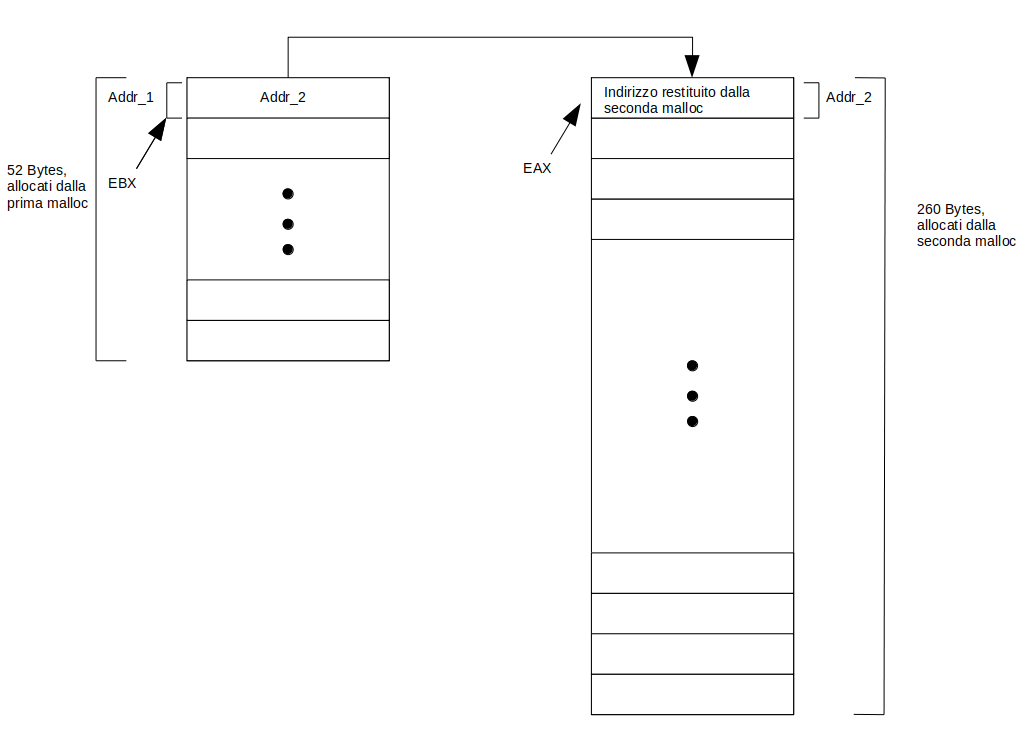
\includegraphics[scale=0.4]{malloc_invocations}\\
In \e{Addr_1}, che è l'indirizzo a cui punta \e{EBX}, è memorizzato un puntatore ad \e{Addr_2}
\end{figure} 

In seguito, viene salvato in \e{EDX} il valore contenuto all'offset \emph{32} con base \e{EBX}; supponendo sia un array di puntatori, si prende l'ottavo.\\
Poi c'è una cosa interessante: la zona di memoria puntata da \e{EAX}, che conserva ancora l'indirizzo restituito dalla seconda \e{malloc}, viene inizializzata a un \e{byte ptr} con valore 0; si sta settando quell'area di memoria a \e{'\tbs0'}. \\
Si procede caricando in \e{ECX} il valore contenuto in \e{EBX+36}: si sta memorizzando il nono elemento. Nell'area puntata da \e{EBX+4} si memorizza il valore 260, in quella puntata da \e{EBX+8} il valore 0. \\

\target{ipotesi}
\textbf{Ipotesi}: sembra che, quella puntata da \e{EBX}, sia una struttura dati in cui il primo campo memorizza un buffer, il secondo la sua grandezza e il terzo i byte effettivamente usati.\\

Il codice continua preparando l'invocazione della funzione
\e{ADVAPI32.DLL::RegQueryInfoKeyA}: vengono messi sullo stack i seguenti parametri (riporati qui nell'ordine in cui li vede la funzione invocata):
\begin{enumerate}
\item Il parametro passato a questa funzione. La documentazione dice che questo è, infatti, l'\emph{handle} verso un registro aperto. È quello ottenuto nella funzione \func{FUN_004018a0_open_handle_to_reg_key}.
\item Il puntatore al buffer memorizzato in \e{EBX}. Questo parametro è opzionale: è un \e{LPSTR} che punta a un buffer che riceve la classe della chiave.
\item Il valore memorizzato nell'area indicizzata da \e{EBX+4}, cioè 260, la dimensione del buffer allocato con la seconda \e{malloc}. Questo è un \e{LPDWORD} che punta a una variabile contenente la dimensione del buffer passato come parametro precedente, come da \func{ipotesi}.
\item Il valore 0. Questo campo è riservato e deve essere \e{NULL}.
\end{enumerate}
\begin{itemize}
\item Vengono passati poi i byte che vanno da \e{EBX+8} a \e{EBX+32}: sono 6 elementi di 4 bytes ciascuno. Sono infatti 6 \e{LPDWORD} che memorizzano, in ordine: 
	\begin{enumerate}
	 \setcounter{enumi}{4}
	\item Un puntatore a una variabile che riceve il numero di sotto-chiavi contenute nella chiave specificata. Non è, come si pensava nell'\func{ipotesi}, il numero di bytes utilizzati.
	\item Un puntatore a una variabile che riceve la dimensione della sotto-chiave con il nome più lungo, senza il terminatore di stringa
	\item Un puntatore a una variabile che riceve la dimensione della stringa più lunga che specifica una classe, anche qui senza terminatore di stringa.
	\item Un puntatore a una variabile che riceve il numero di valori associati alla chiave passata.
	\item Un puntatore a una variabile che riceve la dimensione del nome più lungo tra tutti i valori associati alla chiave.
	\item Un puntatore a una variabile che riceve la dimensione del componente dati più grande tra tutti i valori associati alla chiave, espresso in bytes.
	\end{enumerate}
\end{itemize}
\begin{enumerate}
\setcounter{enumi}{10}
\item Il valore di \e{EBX+32}. Questo è un \e{LPDWORD} e punta a una variabile che riceve la dimensione del \emph{security descriptor} della chiave, in bytes.

\item L'indirizzo di \e{EBX+36}. Questo parametro è un \e{PFILETIME}, che punta a una struttura che riceve l'ultimo istante di tempo in cui la chiave o uno dei suoi valori è stato modificato. Di conseguenza, in \e{EBX+36} è memorizzata una struttura \e{FILETIME}.

\end{enumerate}

Si può quindi definire una struttura dati di 52 byte, che chiamiamo \e{all_subkey_info_keeper}. Questa struttura è, per ora, definita nel seguente modo:
\begin{figure}[H]
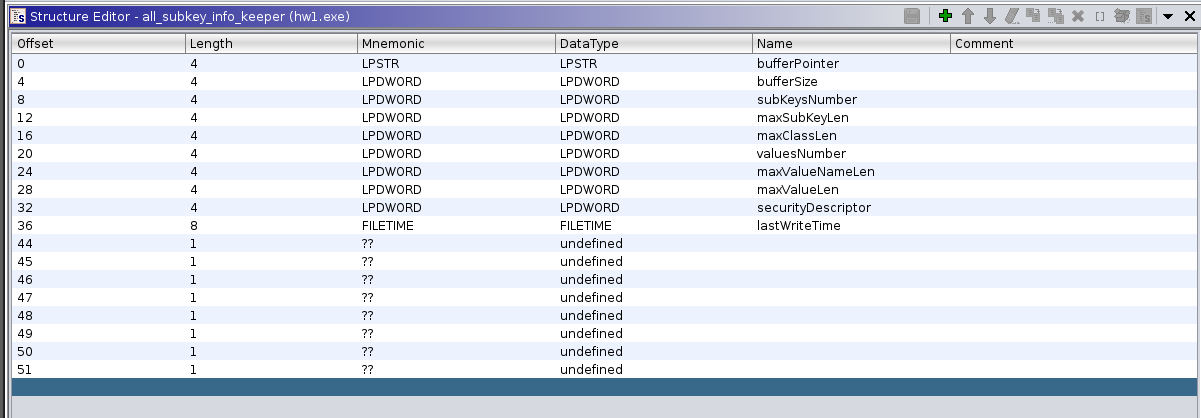
\includegraphics[width=\textwidth]{all_subkey_info_keeper_not_full}\\
Rimangono ancora altri bytes da definire.
\end{figure}


Quando la funzione termina, si controlla il valore di ritorno: se non è 0, viene stampata la stringa \e{"RegQueryInfoKey failed: key not found"} tramite la funzione \e{MSVCRT.DLL::puts} e viene poi ritornato il valore 0.\\
Se la funzione ha avuto successo, invece, si controlla il terzo campo della struttura, e cioè il numero di sotto-chiavi. \\
Se questo valore non è 0 inizia un ciclo che, come prima istruzione, alloca 16 bytes con la funzione \e{malloc}; si salva il valore di ritorno nel registro \e{EBP} e si controlla il suo valore. \\

\nota{i valori restituiti da \e{malloc} sono salvati tutti: in \e{EBX} c'è il primo, ed è la struttra dati di tipo \e{all_subkey_info_keeper}; nel primo campo di \e{EBX} c'è il buffer; e infine questi 16 bytes sono salvati in \e{EBP}.}\\

Se \e{malloc} fallisce, l'esecuzione termina con codice di uscita 1, stampando il messaggio di errore \e{"Memory allocation error"}. Se tutto va bene, invece, si inizializza il valore dei bytes allocati. \\
Anche questa sembra essere una struttura dati: a suggerirlo è il fatto che vengono inizializzati gli indirizzi ottenuti con un offset a partire dall'indirizzo base restituito da \e{malloc}. I campi vengono inizializzati nel seguente modo: 
\begin{figure}[H]
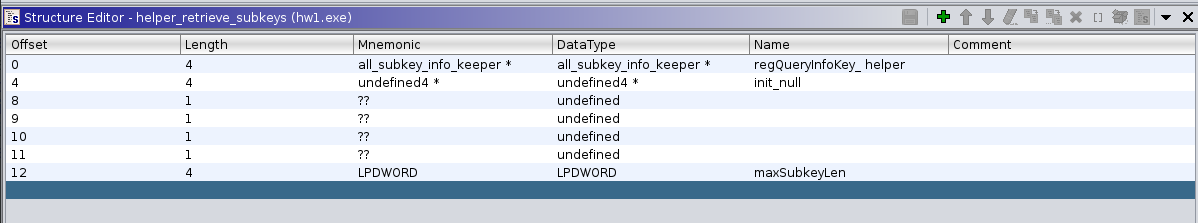
\includegraphics[width=\textwidth]{helper_retrieve_subkeys_not_full}\\
Anche qui rimangono ancora altri bytes da definire e non è ancora chiaro a cosa serva il secondo campo.
\end{figure}
Questa struttura dati, come detto, viene memorizzata in \e{EBP}, e viene rinonimata in \e{helper_retrieve_subkeys}. \bigskip

Il codice continua invocando ancora \e{malloc} e il numero di byte da allocare è pari a \emph{maxSubKeyLen}. Come al solito, si controlla se la funzione ha avuto successo e in caso di fallimento termina l'esecuzione dell'applicazione.\\
Il valore di ritorno viene memorizzato nel terzo campo della struttura in \e{EBP}, ma anche sullo stack, nella variabile \e{local_54}. Il riferimento alla struttura dati in \e{EBP} viene salvato anche in \e{EDI}. Il terzo campo, che era rimasto indefinito, è quindi un puntatore a un'area di memoria della dimensione specificata nel quarto campo, cioè \emph{maxSubKeyLen}. \\
Si prepara l'invocazione della funzione \e{ADVAPI32.DLL::RegEnumKeyExA}, inserendo sullo stack i seguenti valori:
\begin{enumerate}
\item Il primo parametro della funzione, cioè l'handle al registro aperto.
\item Il valore del registro \e{ESI}, impostato precedentemente a 0. Questo valore è un \e{DWORD} che rappresenta l'indice della sottochiave da recuperare. Nella prima invocazione di questa funzione, questo parametro deve essere 0, mentre deve essere poi incrementato per invocazioni successive.
\item Il buffer di \emph{maxSubKeyLen} bytes memorizzato al terzo campo della struttura in \e{EBP}. Infatti questo è un puntatore a un buffer che riceve il nome della sotto-chiave, includendo il terminatore di stringa.
\item Il quarto campo della struttura di tipo \e{helper_retrieve_subkeys}, che rappresenta il puntatore alla dimensione del buffer e, in questo caso, vale \emph{maxSubKeyLen}. La documentazione prevede infatti un pointer a una variabile che specifica la dimensione del buffer passato nel parametro precedente.
\item Il valore 0. Parametro riservato: come da documentazione, è \e{NULL}.
\item Il valore 0. Qui si può avere \Null{} oppure un puntatore a un buffer che riceve una classe della sotto-chiave definita dall'utente.
\item Il valore 0. Anche qui si può avere \Null{}. Se, però, nel parametro precedente c'è un buffer, qui va inserita la sua dimensione.
\item Il valore di \e{ECX}, che contiene l'indirizzo dell'ottavo campo della struttura \e{all_subkey_info_keeper}. Questo parametro è un \e{PFILETIME} in cui verrà inserito l'istante di tempo in cui la sotto-chiave è stata scritta l'ultima volta.
\end{enumerate}

Si controlla il valore di ritorno della funzione: se tutto è andato bene, si incrementa il valore in \e{ESI}: questo registro è usato come secondo parametro di \e{RegEnumKeyExA} e, come detto, deve essere un valore incrementale per indicizzare le varie sotto-chiavi; può essere interpretato come un indice che parte da 0. Si effettua quindi il confronto tra il valore del campo \emph{subKeysNumber} della struttura dati in \e{EBX} e questo valore incrementato. Se \emph{subKeysNumber} è minore o uguale al contatore si esce dal ciclo, perché tutte le chiavi sono state controllate, altrimenti si riparte con una nuova iterazione. Se invece c'è stato un errore, e quindi il valore di ritorno è diverso da 0, si salva il valore contenuto in \e{EBP+0x4} nel registro \e{EDI} e ci si prepara a un'invocazione della funzione \e{MSVCRT.DLL::free}. A questa funzione è passato di \e{EBP}, che punta all'ultima istanza allocata della struttura dati \e{helper_retrieve_subkeys}. Prima della sua invocazione, si incrementa comunque il contatore in \e{ESI}. Dopo la \e{free}, si confronta il valore del campo \emph{subKeysNumber} della struttura dati in \e{EBX} con il valore di \e{ESI}, quindi dell'indice incrementato. Se \emph{subKeysNumber} è maggiore stretto, si riparte con il ciclo, altrimenti si esce. \\

\nota{quando le cose vanno bene, il ciclo ricomincia con \e{EDI} impostato al valore di \e{EBP}, cioè al valore dell'istanza corrente della struttura dati. All'iterazione successiva, viene allocata una nuova istanza della struttura e il secondo campo viene impostato a \e{EDI}, cioè all'istanza precedente. Si sta quindi costruendo una \emph{lista collegata}. \\
Quando le cose vanno male, invece, l'attuale istanza della classe non è inclusa nella catena, e viene anzi rilasciata. Il registro \e{EDI} viene impostato al valore dell'istanza creata all'iterazione precedente, che è appunto memorizzata nel secondo campo della struttura: si sta escludendo dalla catena l'istanza attuale.}\\


Una volta usciti dal ciclo, si memorizza nella struttura dati di \e{EBX}, all'offset \emph{44}, il valore di \e{EAX}: attualmente, in questo registro è salvato il valore di \e{EDI}, che contiene la base della lista collegata. Possiamo quindi definire il campo della struttura dati \e{all_subkey_info_keeper} all'offset \emph{44} come la base della lista collegata delle strutture di tipo \e{helper_retrieve_subkeys}. \\
Se invece nel ciclo non ci si entra proprio, perché il valore di \emph{subKeyNumber} restituito dalla funzione \e{RegQueryInfoKeyA} è pari a 0, allora si memorizzerà il valore \e{NULL}. 

Il codice continua con un controllo sul campo \emph{valuesNumber} della struttura dati \e{all_subkey_info_keeper}. Se il numero dei valori non è 0 inizia un ciclo, dove, per prima cosa, vengono allocati con \e{malloc} la bellezza di 16660 bytes, che corrispondono a circa 16 Megabites e l'indirizzo di ritorno viene memorizzato in \e{EBP}; ovviamente c'è un controllo sul valore restituito e, in caso di errore, si termina mostrando la solita stringa \emph{"Memory allocation error"}. \\

\nota{prima sono state controllate tutte le sotto-chiavi, adesso sta preparando il controllo su tutti i valori associati alla sotto-chiave. È lecito pensare che anche questa sia una struttura dati e che anche qui verrà costruita una lista collegata.} \\

In effetti, la logica è la stessa: viene memorizzato all'offset \emph{4} il valore di \e{ESI}, che contiene inizialmente un puntatore a \Null{}, ma poi conterrà l'istanza della struttura creata all'iterazione precedentemente. In seguito si imposta come primo valore il valore di \e{EBX}, cioè il puntatore alla struttura dati di tipo \e{all_subkey_info_keeper}. Si memorizza poi all'offset \emph{16392} il valore 16383, mentre all'offset \emph{8} si inizializza il terminatore di stringa. Si inserisce all'offset \emph{16656} il valore 256; si sono inizializzati i suoi campi. Chiamiamo questa struttura \e{helper_retrieve_values}. \\

Si prepara poi l'invocazione di \e{ADVAPI32.DLL::RegEnumValueA}: vengono passati sullo stack i seguenti parametri:
\begin{enumerate}
\item Il parametro della funzione, cioè l'handle alla chiave.
\item Il valore 0, contenuto nel registro \e{EDI}. Questo è come il parametro 2 della chiama a \e{RegEnumKeyExA}: è un valore incrementale che indicizza il valore da recuperare.
\item L'indirizzo dell'offset \emph{8} a partire dall'indirizzo allocato con \e{malloc}. Rappresenta un buffer che riceve il nome del valore. Include il terminatore di stringa.
\item L'indirizzo dell'offset \emph{16392} a partire dall'indirizzo della struttura dati \e{helper_retrieve_values}. È un puntatore a un'area di memoria contenente la dimensione del buffer precedente, ma non include il terminatore di stringa. Il valore puntato è inizializzato al valore \emph{16383}, quindi all'offset \emph{8} è contenuto un buffer di \emph{16834} caratteri. Torna con ciò che è stato inserito nella struttura precedentemente.
\item Il valore 0. Parametro riservato e deve essere \e{NULL}
\item L'indirizzo dell'offset \emph{16396}. Puntatore a una variabile che riceve un codice che indica il tipo di dato memorizzato nel valore specificato. Questo sarà, nella struttura, un \e{LPDWORD}.
\item L'indirizzo dell'offset \emph{16400}. Puntatore a un buffer che riceve i dati relativi al valore.
\item L'indirizzo dell'offset \emph{16656}, il cui valore puntato è inizializzato a \emph{256}. Puntatore a una variabile che specifica la dimensione del buffer precedente, in bytes. Quindi l'allocazione di memoria all'offset \emph{16400} è un buffer di \emph{256} bytes. Le dimensioni tornano.
\end{enumerate} 
Quando l'invocazione ritorna, si controlla il suo valore di ritorno. Se è andato tutto bene, il valore \e{EDI}, che è l'indice del valore che viene recuperato, viene incrementato di 1; si controlla quindi che questo valore non sia maggiore del campo all'offset \emph{20} di \e{EBX}, cioè \emph{valuesNumber}. Se il contatore è minore, si riparte nel ciclo, altrimenti si esce. \\
Se invece il valore di ritorno è diverso da zero, si salva il valore di \e{EBP+0x4} nel registro \e{ESI} prima di inserire \e{EBP} sullo stack per invocare la \e{free}: in questo modo si esclude dalla lista collegata l'istanza attuale, che ha generato errore. Si continua poi incrementando il contatore e facendo il controllo nescessario a determinare se uscire dal ciclo o meno.\\

Una volta usciti dal ciclo, si memorizza il valore salvato nel registro \e{ESI}, che contiene la lista collegata appena creata, all'interno dell'offset \e{0x30} di \e{EBX}, che memorizza ancora la struttura dati di tipo \e{RegQueryInfoKey_helper_struct}. Infine, il valore contenuto in questo registro viene ritornato dalla funzione. \\

Le strutture dati, al termine della funzione, sono così definite:
\begin{figure}[H]
\target{all_subkey_info_keeper}
\centering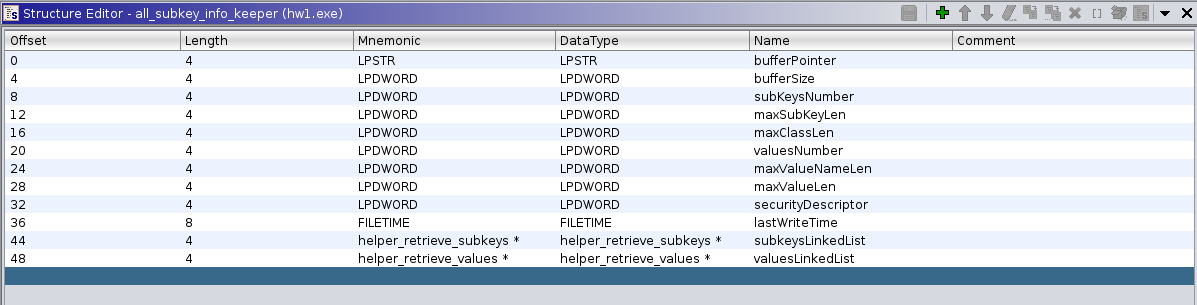
\includegraphics[width=\textwidth]{all_subkey_info_keeper} \\
\end{figure}
\begin{figure}[H]
\centering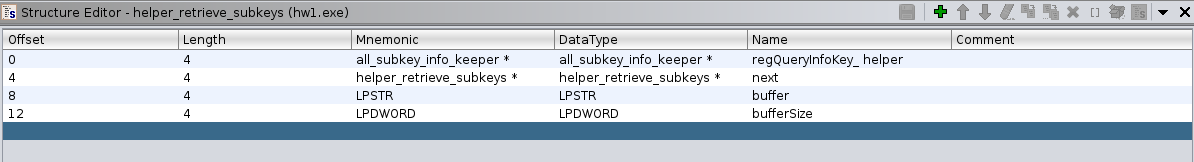
\includegraphics[width=\textwidth]{helper_retrieve_subkeys}\\
\end{figure}
\begin{figure}[H]
\centering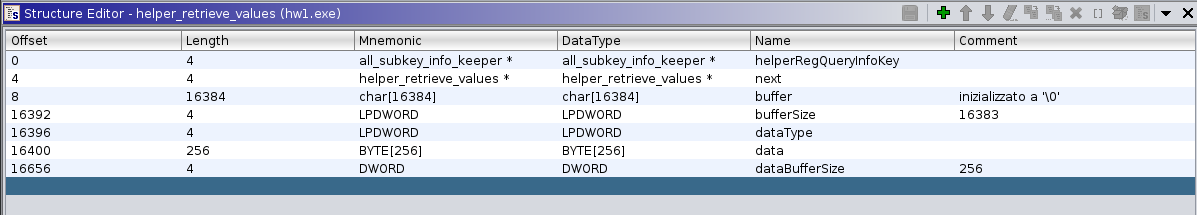
\includegraphics[width=\textwidth]{helper_retrieve_values}\\

\end{figure}

\emph{Riassumendo}: la funzione esplora la chiave passata in input per cercare i valori e le sotto-chiavi ad essa collegate. Memorizza il tutto in una struttura dati che viene poi ritornata. In particolare, nella struttura dati ritornata ci sono due campi che memorizzano le \emph{liste collegate} rispettivamente di sotto-chiavi e valori che non hanno generato errori durante la loro analisi.\\
Questa funzione, terminando, restituisce il controllo a \func{FUN_004018a0_open_handle_to_reg_key} che, a questo punto, non fa altro che restituire al \e{main} la struttura dati \e{all_subkey_info_keeper} creata.



\target{FUN\_00401790\_print\_catched\_info}
\target{FUN\_00401790}
\subsection{FUN\_00401790\_print\_catched\_info}
Questa funzione è l'ultima invocata dal \verb+main+ che non è stata ancora analizzata. Prende in input il valore ritornato da \func{FUN_004018a0_open_handle_to_reg_key}, che è un puntatore a \func{all_subkey_info_keeper}.\\
Per analizzare questa funzione, conviene guardare il decompilato: risulta infatti molto chiaro che questa funzione ha lo scopo di stampare tutto ciò che è stato precedentemente creato e salvato nella struttura dati passata come primo parametro. \\

\end{document}
